\noindent  \textbf{Información inicial}:
\begin{multicols}{2}
	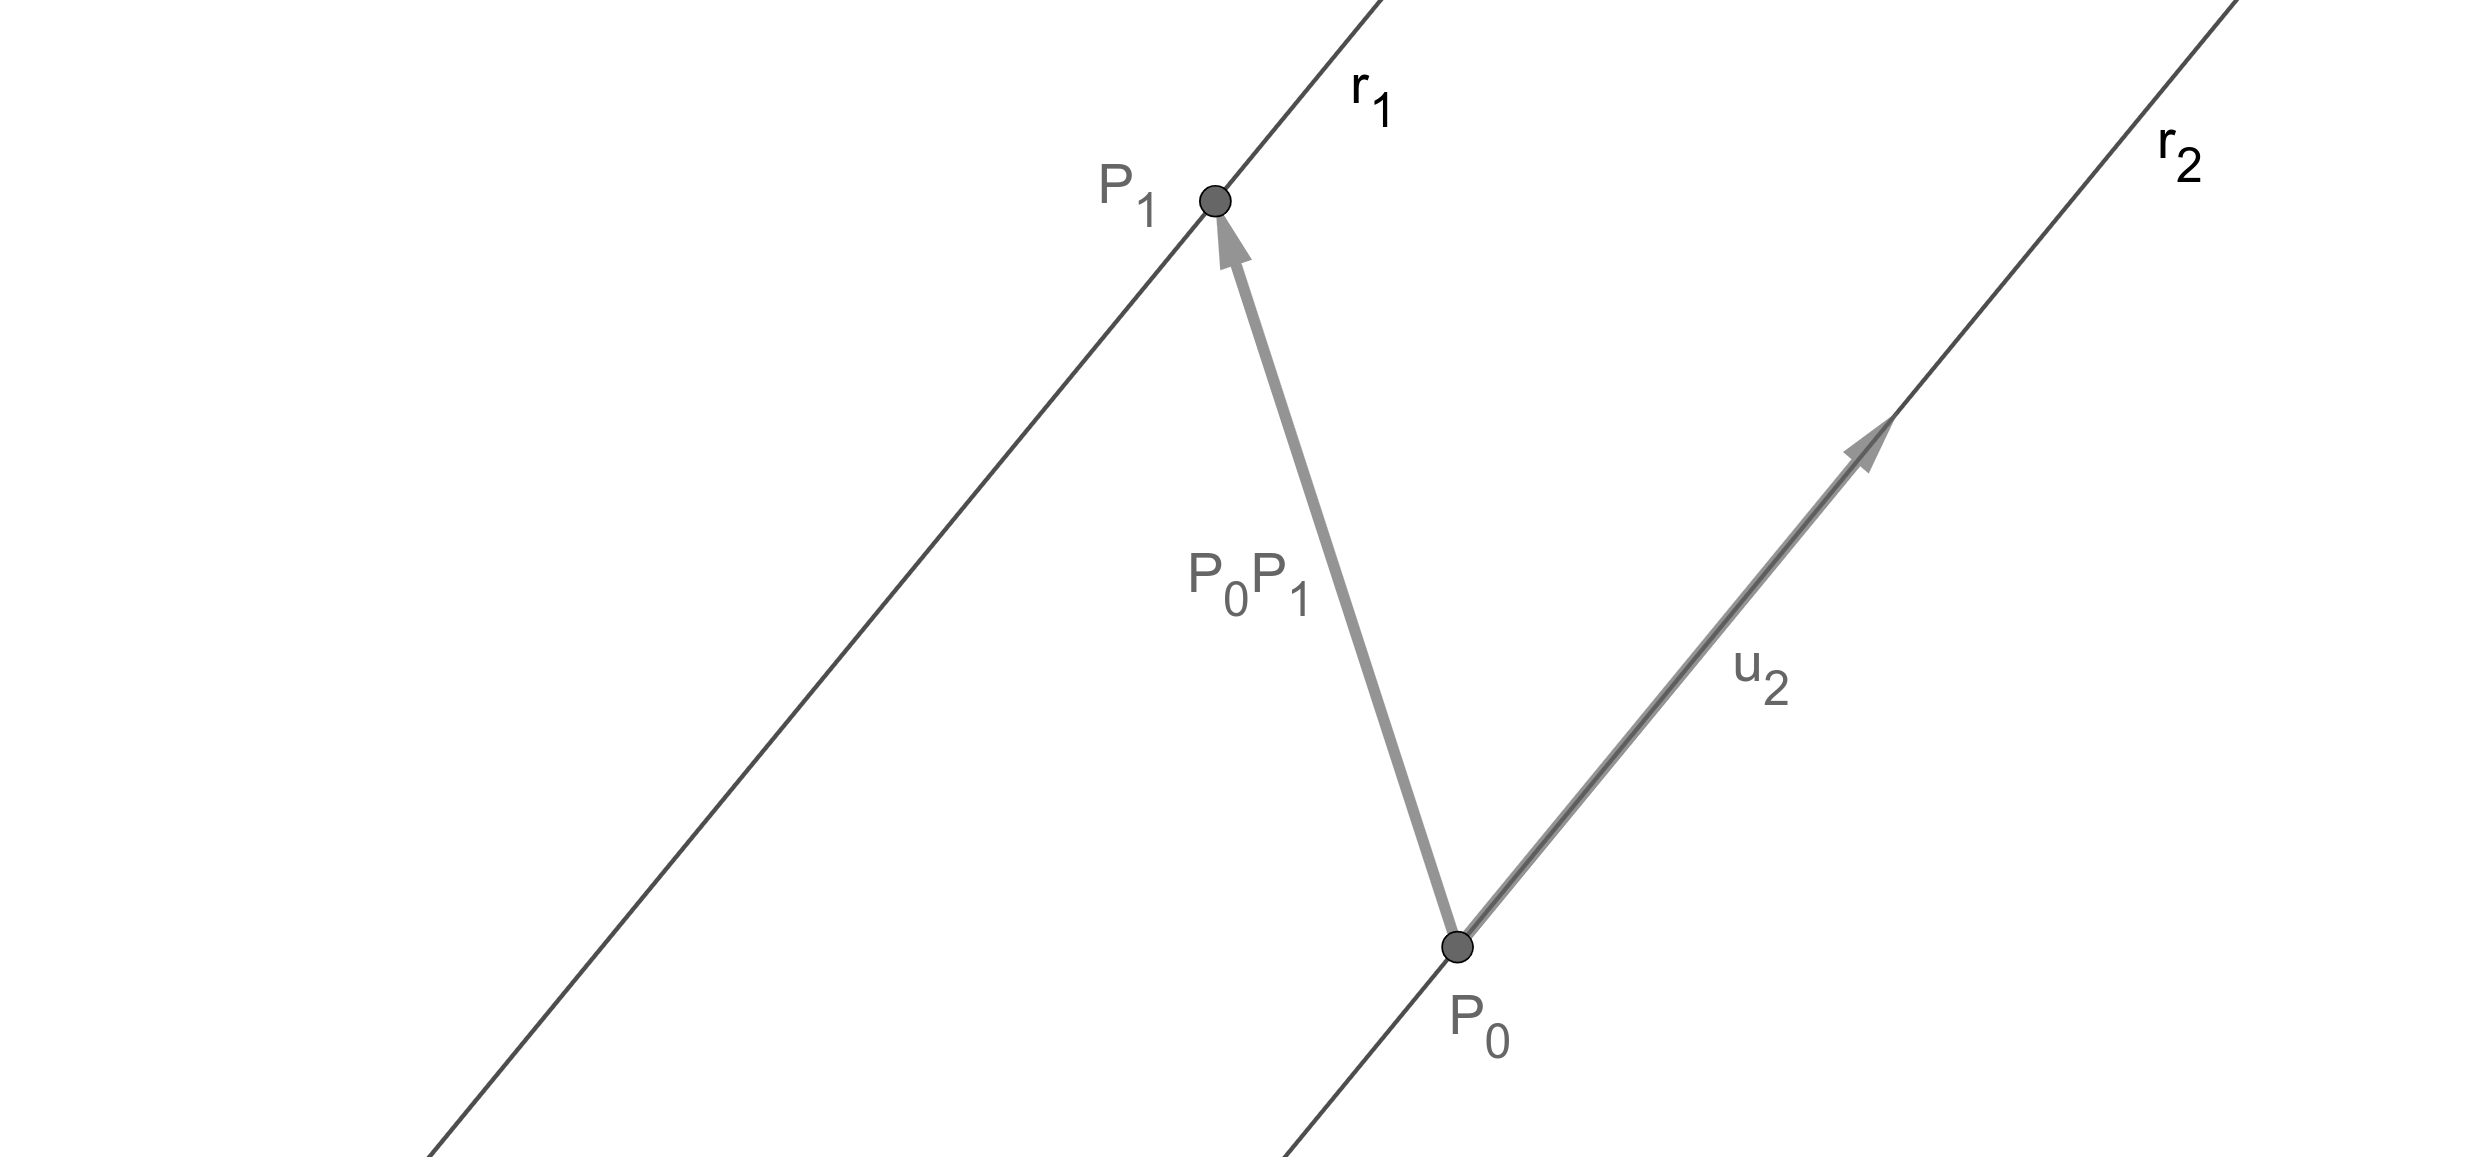
\includegraphics[width=7cm, scale=0.8]{12b1.png} \\
	$\overrightarrow{P_0P_1} \times \vec{u_2} = \vec{n}$, vector normal al plano determinado por $\overrightarrow{P_0P_1}$ y $\vec{u_2}$.
\end{multicols}

\noindent \textbf{Buscamos un punto de paso $P_1$ en $r1$}:
\begin{multicols}{2}
	\noindent Si $z=\boxed{0} \implies \begin{cases}
			3x - 2y - 5 = 0 \hspace{0.5cm} (1) \\
			2x + y - 5 = 0 \hfill (2)
		\end{cases}$

	\noindent Despejamos $y$ de $(1)$:
	\begin{align*}
		3x - 2y - 5 & = 0                                    \\
		-2y         & = -3x + 5                              \\
		y           & = \dfrac{-(3x - 5)}{-2}                \\
		y           & = \dfrac{3x - 5}{2} \hspace{0.5cm} (3)
	\end{align*}

	\noindent Reemplazamos $(3)$ en $(2)$ para hallar $x$:
	\begin{align*}
		2x + y - 5                                & = 0                    \\
		2x + \left( \dfrac{3x - 5}{2} \right) - 5 & = 0                    \\
		2x + \dfrac{3x}{2} - \dfrac{5}{2} -5      & =0                     \\
		\dfrac{7}{2}x - \dfrac{15}{2}             & = 0                    \\
		7x - 15                                   & = 0                    \\
		x                                         & =\boxed{\dfrac{15}{7}}
	\end{align*}

	Reemplazamos $x$ en $(3)$ para hallar $y$:
	\begin{align*}
		y & = \dfrac{3x - 5}{2}                                      \\
		y & = \dfrac{3}{2}x - \dfrac{5}{2}                           \\
		y & = \dfrac{3}{2} \left(\frac{15}{7} \right) - \dfrac{5}{2} \\
		y & = \dfrac{45}{14} - \dfrac{35}{14}                        \\
		y & = \dfrac{10}{14}                                         \\
		y & = \boxed{\dfrac{5}{7}}                                   \\
	\end{align*}

	$\therefore \ \boxed{P_1 \left (\frac{15}{7}, \frac{5}{7}, 0 \right) \in r1}$
\end{multicols}

\vspace{6cm}
%\vfill
\noindent \textbf{A partir de este punto de paso $P_1$ podemos buscar el vector $\vec{n}$ del plano determinado por $r1$ y $r2$}:

\begin{center}
	$P_0(1, 3, -2) \hspace{1cm} P_1 \left (\frac{15}{7}, \frac{5}{7}, 0 \right)$
\end{center}

%\newpage
\noindent Armamos el vector $\overrightarrow{P_0P_1}$:
\begin{align*}
	\overrightarrow{P_0P_1} & = \left (\frac{15}{7}, \frac{5}{7}, 0 \right) - (1, 3, -2)       \\
	\overrightarrow{P_0P_1} & = \left (\frac{15}{7} - 1, \ \frac{5}{7} - 3, \ 0 - (-2) \right) \\
	\overrightarrow{P_0P_1} & = \left (\frac{8}{7}, \ -\frac{16}{7}, \ 2 \right)               \\
\end{align*}

\noindent Buscamos el vector $\vec{n}$ con $\overrightarrow{P_0P_1}$ y $\vec{u_2}$:
\begin{align*}
	\vec{n}              & = \overrightarrow{P_0P_1} \times \vec{u_2}                         \\
	\vec{n}              & = \begin{vmatrix}
		                          i           & j             & k  \\
		                          \frac{8}{7} & -\frac{16}{7} & 2  \\
		                          2           & 10            & 14
	                          \end{vmatrix}                                 \\
	\vec{n}              & = \vec{i} \left[(-\frac{16}{7})\cdot(14) - (2)\cdot(10) \right]  +
	\vec{j} \left[ (2)\cdot(2) - (\frac{8}{7})\cdot(14) \right] +
	\vec{k} \left[ (\frac{8}{7})\cdot(10) - (-\frac{16}{7})\cdot(2) \right]                    \\
	\vec{n}              & = \vec{i} \left[-32 - 20 \right]  +
	\vec{j} \left[ 4 - 16 \right] +
	\vec{k} \left[ \frac{80}{7} + \frac{32}{7} \right]                                         \\
	\vec{n}              & = \vec{i} (-52) + \vec{j} (- 12) + \vec{k} (16)                    \\
	\vec{n}              & = -52\vec{i}- 12\vec{j} + 16\vec{k}                                \\
	\vec{n}              & = -13\vec{i}- 3\vec{j} + 4\vec{k}                                  \\
	\therefore \ \vec{n} & = \boxed{(-13, -3, 4)}
\end{align*}

\noindent Con el vector $\vec{n}$ encontrado empezamos a armar la ecuación del plano al que llamaremos $\omega$:
\begin{center}
	$\omega) \hspace{1cm} -13x - 3y + 4z + d = 0$
\end{center}

\noindent Usamos el punto $P_0(1, 3, -2)$ para determinar el valor de $d$:
\begin{align*}
	-13x - 3y + 4z + d        & = 0          \\
	-13(1) - 3(3) + 4(-2) + d & = 0          \\
	-13 - 9 - 8 + d           & = 0          \\
	-30 + d                   & = 0          \\
	d                         & = \boxed{30}
\end{align*}

\noindent $\therefore \ \fcolorbox{black}{yellow}{$\omega) \ \ -13x - 3y + 4z + 30 = 0$}$ es la ecuación del plano determinado por las rectas $r1$ y $r2$.

\vspace{2cm}
\noindent \textbf{Gráfica 12-b}:
\begin{center}
	\href{https://www.geogebra.org/3d/n89vhber}{\includegraphics[width=15cm, scale=1]{TP-MATEMÁTICA-EJ12B.png}}
\end{center}